%arara: lualatex: { branch: developer, interaction: errorstopmode,
%arara: --> shell: yes, synctex: yes }
%arara: biber: { options: [ '--wraplines' ] }

% \DocumentMetadata{testphase=phase-III}
\DocumentMetadata{lang=es-MX}

% NOTA: [<+->] se usa comio overlay para hacer que los bullets aparezcan uno por uno.


\documentclass[%
spanish,
    progressbar=head,
background=dark,
subsectionpage
]{beamer}

\usepackage{babel}
\usepackage{microtype} 
\usepackage{tabularray}
\UseTblrLibrary{booktabs}
\usepackage{siunitx}
\usepackage{chemmacros}
\usepackage{multimedia}


\usepackage[style=authoryear,backend=biber]{biblatex}
    \addbibresource{Bibliografia.bib}


\usepackage[skins]{tcolorbox}
    \tcbset{skin=beamer}

\usepackage{pgf}

\newcommand{\includemaskedgraphics}[2][]{%
    \IfFileExists{#2-mask.png}{}{\immediate\write18{convert #2.jpg -alpha set -channel RGBA -fuzz 3\% -fill none -floodfill +0+0 white -channel RGBA -separate +channel -evaluate-sequence add -threshold 0 -colorspace GRAY -negate #2-mask.png}}
    \pgfdeclaremask{themask}{#2-mask.png}
    \pgfimage[#1, mask=themask]{#2.jpg}
}

\usepackage{pgfpages}
\setbeamertemplate{note page}[plain]
% \setbeameroption{show notes on second screen=right}

\usetheme{metropolis}

% \usecolortheme{orchid}
% \title{Técnicas de preparación de materiales}
\title{Aleaciones mecánicas}
\subtitle{Variables del proceso de molienda}
\date{\today}
\author{Pablo E. Alanis}
\institute{Universidad Autónoma de Nuevo Leon, División de Posgrado\\Técnicas de preparación de materiales}
\begin{document}
\maketitle

\section{Variables del proceso}
\begin{frame}{Aleaciones mecánicas | Variables del proceso}
    \begin{columns}
    \column[c]{0.3\linewidth}
    \begin{itemize}
        \item<1-> El proceso de \emph{aleación mecanica} es complejo;
        \item<2-> para obtener el producto deseado, se tienen que \textit{optimizar} las condiciones de reacción.
    \end{itemize}
    \column[c]{0.7\linewidth}
    \begin{figure}
        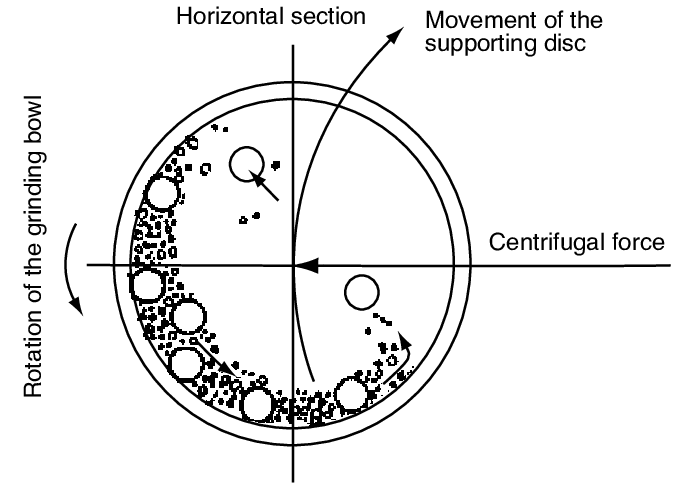
\includegraphics[width=\linewidth]{figuras/milling.png}
        \caption{Esquema del proceso de molienda en un molino de bolas.}
    \end{figure}
\end{columns}
    % \column[c]{0.7\linewidth}
    % \begin{figure}
    %     \begin{center}
    %     \begin{overprint}
    %         \onslide<1> 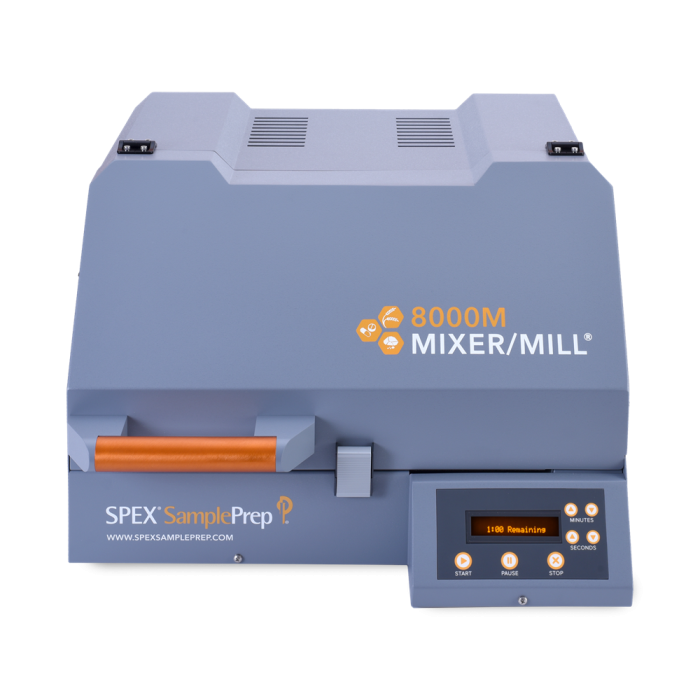
\includegraphics[width=\linewidth]{figuras/big.png} \note<1>{Este es un molino de bolas SPEX}
    %         \onslide<2> 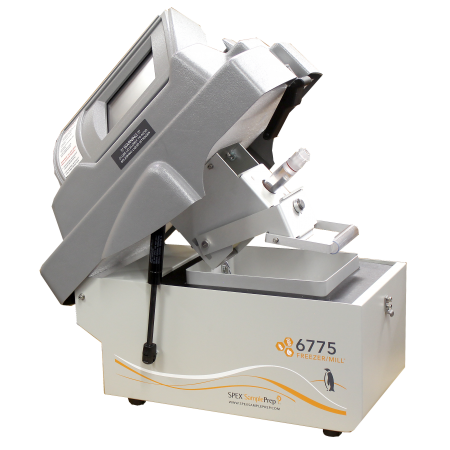
\includegraphics[width=\linewidth]{figuras/cryo.png}
    %         \note<2>{Este es un molino SPEX con capacidad de mantener temperaturas criogénicas.}
    %     \end{overprint}
    %     \end{center}
    % \end{figure}
    % \end{columns}
\end{frame}

\begin{frame}{Aleaciones mecánicas | Variables del proceso}
    Entre algunas de las variables que afectan la fase del producto final obtenido, se encuentran:

    \begin{itemize}
        \item \emph{tipo} de molino;
        \item \emph{contenedor} del molino;
        \item \emph{velocidad} de molienda;
        \item \emph{tiempo} de molienda;
        \item \emph{tipo, tamaño y distribución} del medio de molienda;
        \item \emph{relación} en masa de bolas-polvo;
        \item \emph{que tan lleno} está el vial;
        \item \emph{atmósfera} de molienda;
        \item \emph{agente de control} del proceso;
        \item \emph{temperatura} de molienda.
    \end{itemize}
\end{frame}

\begin{frame}{Aleaciones mecánicas | Variables del proceso}
\begin{itemize}
    \item Estas variables no son necesariamente independientes;\\
    \item[] \textbf{por ejemplo:} el tiempo de molienda óptimo puede depender de: 
    \begin{enumerate}
        \item tipo de molino;
        \item tamaño del medio de molienda;
        \item temperatura de molienda;
        \item relación bolas-polvo, etc.
    \end{enumerate}
\end{itemize}
\end{frame}

\begin{frame}{Aleaciones mecánicas | Variables del proceso}
    \begin{itemize}
        \item Estas variables no son necesariamente independientes;\\
        \item[] \textbf{por ejemplo:} el tiempo de molienda óptimo puede depender de: 
        \begin{enumerate}
            \item tipo de molino;
            \item tamaño del medio de molienda;
            \item temperatura de molienda;
            \item relación bolas-polvo, etc.
        \end{enumerate}
    \end{itemize}
\end{frame}

\subsection{Tipo de molino}

\begin{frame}{Tipos de molinos}
    \begin{itemize}
        \item Existen varios tipos de molinos que pueden usarse según el propósito;
        \item Estos varían en:
            \begin{enumerate} 
                \item capacidad;
                \item velocidad de operación;
                \item capacidad para controlar la temperatura.
            \end{enumerate}
    \end{itemize}
\end{frame}

\begin{frame}{Capacidades de los molinos}
    Según la cantidad de polvo que se requiera sintetizar, se pueden utilizar diferentes molinos:
    \begin{itemize}
        \item \textbf{Para propositos de \emph{screening}} se puede utilizar un molino tipo \emph{SPEX.}
        \item \textbf{Para producir grandes cantidades de polvo} se puede utilizar un molino tipo Fristsch Pulverisette planetario.
    \end{itemize}
\end{frame}

\begin{frame}{Capacidades de los molinos --- Comparación}
\begin{longtblr}[%
    caption = {\small Comparación de tipos de molinos convencionales en función a cantidades de material que pueden procesar.},
    % entry = {Short Caption},
    label = {tbl:TipoDeMolino}]
    {%
    colspec = {XX}, width = 0.85\linewidth,
    rowhead = 1
    }
    \toprule
    Tipo de molino & Tamaño de muestra \\ \midrule
    Molino mezclador & Hasta dos de \qty{20}{\gram} \\
    Molino planetario & Hasta cuatro de \qty{250}{\gram} \\
    Attritores & \qtyrange{0.5}{100}{\kilo\gram} \\
    Molinos Uni-ball & Hasta cuatro de \qty{2000}{\gram} \\ \bottomrule
\end{longtblr}
\end{frame}

\subsection{Tipo de molino}

\begin{frame}{Contenedor del molino}
\begin{itemize}
    \item El material del contenedor del molino es un factor muy importante a considerar.
    \begin{enumerate}
        \item Puede influir en que tan contaminada pueda estar nuestra fase metaestable.
        \item Si ambos tiene el mismo material, puede alterar la composición química del polvo.
    \end{enumerate}
\end{itemize}
\end{frame}

\begin{frame}{Materiales convencionales}
    Entre los materiales mas comunes para contenedores con aplicaciones en molinos se encuentran:
    \begin{itemize}
        \item acero reforzado;
        \item acero cromado reforzado;
        \item acero templado;
        \item acero inoxidable;
        \item \ch{WC-Co}
        \item acero cubierto de WC.
    \end{itemize}
\end{frame}

\begin{frame}{Materiales para propósitos especiales}
    \begin{columns}\note{Se pueden usar contenedores de materiales especializados}
        \column{0.38\linewidth}
        \small
    Contenedores de materiales para propósitos especializados:
    \begin{itemize}
        \item<1-> cobre;
        \item<2-> titanio;
        \item<3-> safíro;
        \item<4-> agata;
        \item<5-> porcelana dura;
        \item<6-> \ch{Si3N4}
        \item<7-> \ch{Cu-Be}
    \end{itemize}
    \column[c]{0.58\linewidth}
    \begin{figure}
        \begin{center}
        \begin{overprint}
            \onslide <1>\pgfimage[width=\linewidth]{./figuras/materiales/cu.jpg}
            \onslide <2>\pgfimage[width=\linewidth]{./figuras/materiales/ti.jpg}
            \onslide<3>\pgfimage[width=\linewidth]{./figuras/materiales/zap.jpg}
            \onslide<4>\pgfimage[width=\linewidth]{./figuras/materiales/aga.jpeg}
            \onslide<5>\pgfimage[width=\linewidth]{./figuras/materiales/por.jpg}
            \onslide<6>\pgfimage[width=\linewidth]{./figuras/materiales/sin.png}
            \onslide<7>\pgfimage[width=\linewidth]{./figuras/materiales/cube.jpg}
        \end{overprint}
        \end{center}
    \end{figure}
    \end{columns}
\end{frame}

\begin{frame}{Forma del contenedor}
\begin{itemize}
    \item<1-> La forma del contenedor puede afectar en los tiempos de molienda drasticamente.
    \item<2-> para los molinos SPEX existen \emph{contenedores de fondo plano} y \emph{contenedores de fondo redondo}
    \item<3-> El tiempo requerido para que se llegara a la misma intensidad en un pico en XRD en (111) fue de:
    \begin{enumerate}
        \item \qty{9}{\hour} en el contenedor de fondo plano;
        \item \qty{15}{\hour} en el contenedor de fondo redondo.
    \end{enumerate}
\end{itemize}
\end{frame}
%HOLA
\begin{frame}
    \begin{figure}{Forma del contendor}
        \centering
        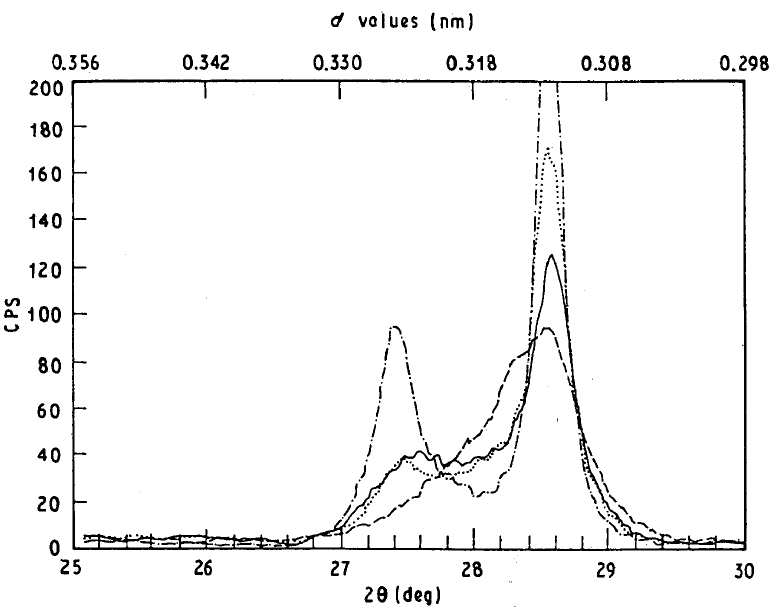
\includegraphics[width=0.85\linewidth]{figuras/efectoXRD.png}
        \caption{Efecto del uso de un contenedor de fondo plano vs uno de fondo redondo \textit{(Obtenido de \cite{harringa1992effects})}}
    \end{figure}
\end{frame}

\begin{frame}{Velocidad de molienda}
    \begin{tcolorbox}[title={Velocidad crítica, \(C_s\):}]
        \small
        En un molino de bolas, la \emph{velocidad crítica (\(C_s\))} es la velocidad en la que el medio de molienda se adhiere, a causa de la fuerza centrífuga, a las paredes del contenedor.
        
        La fórmula de la velocidad crítica es:

        \begin{equation}
            C_s = \frac{\pi}{2}\sqrt{\frac{g}{R-r}}
        \end{equation}

        Donde \(g\) es la constante gravitacional, \(R\) es el diámetro interno del molino y \(r\) el diámetro de un trozo de medio de molienda. 
    \end{tcolorbox}
\end{frame}

\begin{frame}
    \begin{itemize}
        \item<1-> A velocidades mayores que la \textit{velocidad crítica} las bolas estarían sujetas al contenedor y no causarían ningún impacto;
        \item<2-> la velocidad debe ser ajustada para que sea menor que la \emph{velocidad crítica.} 
    \end{itemize}

    \begin{figure}
        \centering
        \includegraphics<1->[width=0.9\linewidth]{figuras/Cs/vel1.jpeg}
    \end{figure}
\end{frame}

\begin{frame}{Velocidad de molienda}
    \begin{itemize}
        \item Los molinos de bolas secos operan en un rango de \qtyrange{50}{70}{\percent} de la \(C_s\);
        \item normalmente se operan de \qtyrange{60}{65}{\percent};
        \begin{enumerate}
            \item a \qty{\le 50}{\percent} \(C_s\) la enrgía es muy poca para \emph{fracturar el polvo;}
            \item a \qty{\geq 70}{\percent} \(C_s\) el medio comienza a caer en \emph{catarata,} golpenado una sola zona del contenedor.
        \end{enumerate}
    \end{itemize} 
\end{frame}

\begin{frame}{Velocidad de molienda | Temperatura del medio}
    Una de las consequencias de moler a \emph{altas velocidades} es que la \emph{temperatura del medio aumenta.}

    En ciertos casos es provechoso:
    \begin{itemize}
        \item promover la homogeneidad y/o aleaciones de polvos.
    \end{itemize}

\end{frame}

\begin{frame}
    O bien, puede ser un problema:
            \begin{itemize}[<+-| alert@+>]
                \item acelera la transformación del proceso, resultando en descomposición de la fase deseada;
                \item se pueden formar otras fases metaestables indeseadas;
                \item incrementa el riesgo de contaminación de polvos.
            \end{itemize}
\end{frame}

\begin{frame}
    % \transfade
    En algunas investigaciones, se han reportado \emph{cambios en la morfología} en función de la \emph{velocidad}:\footcite{calka1991}\note{En algunas investigaciones se ha reoprtado que a diferentes velocidades se producen diferentes fases}
    \medskip
    \begin{longtblr}[caption={Relación de la velocidad con las fases obtenidas}]{colspec = {XX}, width = 0.85\linewidth, rowhead = 1}
    \toprule 
    Fase obtenida & Velocidad de molienda \\ \midrule
    \ch{Ni-Zr} (amorfo) & Alta velocidad \\
    \ch{Ni-Zr} (cristalíno) & Velocidad media y baja \\
    \bottomrule    
    \end{longtblr}
\end{frame}


\begin{frame}[allowframebreaks]{Referencias}
    \small
    \printbibliography
\end{frame}

\end{document}